\documentclass[tikz,border=10pt]{standalone}
\usetikzlibrary{arrows.meta, positioning, calc}

% ---------------------------------------------------------------- colours
\definecolor{c1}{HTML}{15173D}   % the querying word, the rows
\definecolor{c2}{HTML}{982598}   % the word being read, the columns, the cells
\definecolor{c3}{HTML}{E491C9}
\definecolor{c4}{HTML}{F1E9E9}
\definecolor{axiscolor}{HTML}{333333}
\definecolor{labelcolor}{HTML}{6B6472}

% ================================================================
% Geometry, decided before any TikZ was written.
%
%   one grid: pitch 0.95, cell 0.86, gap 0.09
%   column j (0..4) spans x = 0.95j+0.045 .. 0.95j+0.905, centre 0.95j+0.475
%   row    i (0..4) spans y = -0.95i-0.045 .. -0.95i-0.905, centre -0.95i-0.475
%   so each grid occupies x in [0, 4.75], y in [-4.75, 0]
%
%   row labels: anchor east at x = -0.16, in c1
%   column labels: rotated 45, anchor south west at (colcentre-0.10, 0.10), in c2
%       "(3) chased" at scriptsize is about 1.6cm long -> header reaches y ~ 1.25
%   panel title: anchor south, centred on the grid, at y = 1.55, labelcolor
%
%   left panel  dx = 0     (all 25 cells filled)
%   right panel dx = 8.4   (j > i struck out)
%   widest row label "(3) chased" ~ 1.6cm, so the right panel's labels start at
%   x = 8.4-1.76 = 6.64, leaving a 1.9cm clear gap after the left grid at 4.75
%
%   row (3) frame: i = 2, y from -1.855 to -2.895, outset 0.09
%       left  x from -0.09 to 4.84   (five cells)
%       right x from -0.09 to 2.94   (three cells)
%
%   legend line, centred under both panels, at y = -5.35
%   bounding box roughly x in [-1.8, 13.2], y in [-5.8, 2.1]: wide and short
% ================================================================

\newcommand{\pit}{0.95}

\begin{document}
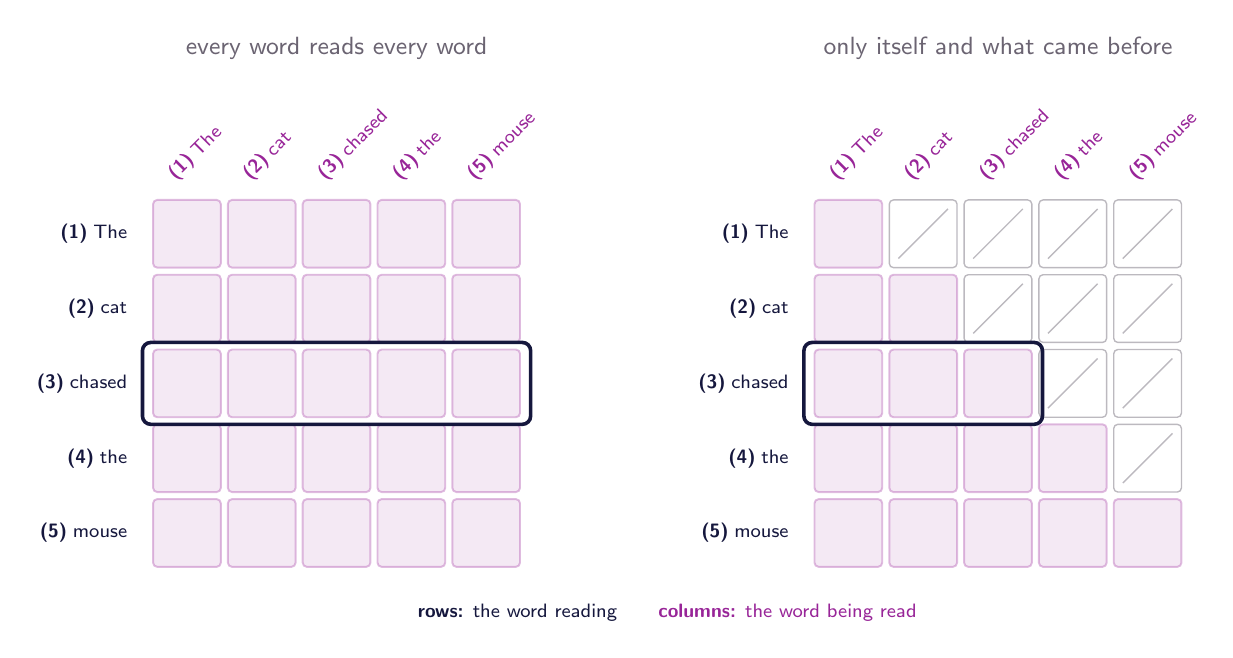
\begin{tikzpicture}[
    every node/.style={font=\sffamily},
    keep/.style={fill=c2, fill opacity=0.10, draw=c2, draw opacity=0.30,
                 line width=0.7pt, rounded corners=1.5pt},
    gone/.style={draw=labelcolor, draw opacity=0.45, line width=0.5pt,
                 rounded corners=1.5pt},
    strike/.style={draw=labelcolor, draw opacity=0.45, line width=0.5pt},
    rowlab/.style={font=\sffamily\scriptsize, text=c1, anchor=east},
    collab/.style={font=\sffamily\scriptsize, text=c2, anchor=south west,
                   rotate=45, inner sep=1pt},
    title/.style={font=\sffamily\small, text=labelcolor, anchor=south},
    frame/.style={draw=c1, line width=1.3pt, rounded corners=3pt},
]

% ---------------------------------------------------------------- the cells
% left panel: every word reads every word
\foreach \i in {0,...,4} {
    \foreach \j in {0,...,4} {
        \draw[keep] ({\pit*\j+0.045}, {-\pit*\i-0.045})
            rectangle ++(0.86, -0.86);
    }
}

% right panel: only itself and what came before
\foreach \i in {0,...,4} {
    \foreach \j in {0,...,4} {
        \ifnum\j>\i
            \draw[gone] ({8.4+\pit*\j+0.045}, {-\pit*\i-0.045})
                rectangle ++(0.86, -0.86);
            \draw[strike] ({8.4+\pit*\j+0.16}, {-\pit*\i-0.79})
                -- ++(0.63, 0.63);
        \else
            \draw[keep] ({8.4+\pit*\j+0.045}, {-\pit*\i-0.045})
                rectangle ++(0.86, -0.86);
        \fi
    }
}

% ---------------------------------------------------------------- labels
\foreach \i/\w in {0/The, 1/cat, 2/chased, 3/the, 4/mouse} {
    \pgfmathtruncatemacro{\p}{\i+1}
    \foreach \dx in {0, 8.4} {
        \node[rowlab] at ({\dx-0.16}, {-\pit*\i-0.475})
            {\textbf{(\p)}\;\w};
    }
    % same list serves the columns
    \foreach \dx in {0, 8.4} {
        \node[collab] at ({\dx+\pit*\i+0.37}, 0.10)
            {\textbf{(\p)}\;\w};
    }
}

% ---------------------------------------------------------------- row (3)
\draw[frame] (-0.09, -1.855) rectangle (4.84, -2.895);
\draw[frame] (8.31, -1.855) rectangle (11.34, -2.895);

% ---------------------------------------------------------------- titles
\node[title] at (2.375, 1.62) {every word reads every word};
\node[title] at (10.775, 1.62) {only itself and what came before};

% ---------------------------------------------------------------- legend
\node[font=\sffamily\scriptsize, anchor=north] at (6.575, -5.05)
    {\textcolor{c1}{\textbf{rows:} the word reading}\qquad
     \textcolor{c2}{\textbf{columns:} the word being read}};

\end{tikzpicture}
\end{document}
